\documentclass[tikz,border=10pt]{standalone}
\usepackage{tikz}
\usetikzlibrary{chains,positioning}

\begin{document}
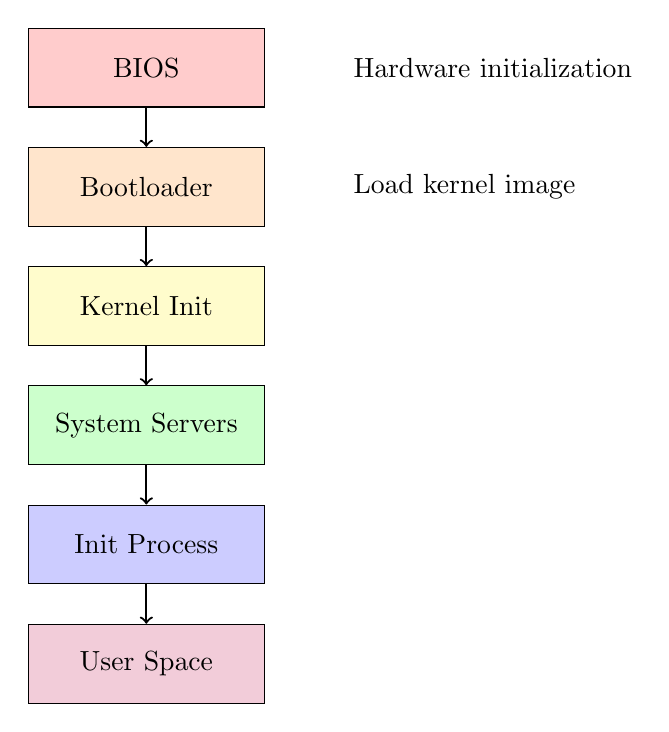
\begin{tikzpicture}[
    stage/.style={rectangle, draw, minimum width=3cm, minimum height=1cm, on chain},
    arrow/.style={->, thick}
]

% Boot stages
\begin{scope}[start chain=going below, node distance=5mm]
    \node[stage, fill=red!20] (BIOS) {BIOS};\n    \node[stage, fill=orange!20, below=of BIOS] (Bootloader) {Bootloader};\n    \node[stage, fill=yellow!20, below=of Bootloader] (KernelInit) {Kernel Init};\n    \node[stage, fill=green!20, below=of KernelInit] (SystemServers) {System Servers};\n    \node[stage, fill=blue!20, below=of SystemServers] (InitProcess) {Init Process};\n    \node[stage, fill=purple!20, below=of InitProcess] (UserSpace) {User Space};
\end{scope}

% Descriptions
\node[right=1cm of BIOS] {Hardware initialization};\n\node[right=1cm of Bootloader] {Load kernel image};

% Connections
\draw[arrow] (BIOS) -- (Bootloader);\n\draw[arrow] (Bootloader) -- (KernelInit);\n\draw[arrow] (KernelInit) -- (SystemServers);\n\draw[arrow] (SystemServers) -- (InitProcess);\n\draw[arrow] (InitProcess) -- (UserSpace);

\end{tikzpicture}
\end{document}